
%--------------------------------------------------------------------
%--------------------------------------------------------------------
% Formato para los talleres del curso de Métodos Computacionales
% Universidad de los Andes
%--------------------------------------------------------------------
%--------------------------------------------------------------------

\documentclass[11pt,letterpaper]{exam}
\usepackage{amsmath}
\usepackage[utf8]{inputenc}
\usepackage[spanish]{babel}
\usepackage{graphicx}
\usepackage{tabularx}
\usepackage[absolute]{textpos} % Para poner una imagen completa en la portada
\usepackage{hyperref}
\usepackage{float}

\newcommand{\base}[1]{\underline{\hspace{#1}}}
\boxedpoints
\pointname{ pt}

\extraheadheight{-0.15in}

\newcommand\upquote[1]{\textquotesingle#1\textquotesingle} % To fix straight quotes in verbatim



\begin{document}
\begin{center}
{\Large M\'etodos Computacionales} \\
Tarea 1 - \textsc{Python}\\
12-08-2016\\
\end{center}

\begin{textblock*}{40mm}(10mm,20mm)
  
\includegraphics[width=3cm]{logoUniandes.png}
\end{textblock*}

\begin{textblock*}{40mm}(164mm,20mm)
  
\includegraphics[width=3cm]{logoUniandes.png}
\end{textblock*}

\vspace{0.3cm}

\noindent
La solución a este taller debe subirse por SICUA antes de las 8:00AM
del jueves 1 de septiembre del 2016. 
\noindent

(10 pt) Los archivos del c\'odigo  deben subirse en un
\'unico archivo \verb".zip" con el nombre
\verb"NombreApellido_hw1.zip", por ejemplo yo deber\'ia subir el zip
\verb"JaimeForero_hw1.zip" al descomprimir el zip debe crearse la
carpeta \verb"JaimeForero_hw1" y adentro debe estar el c\'odigo.


\vspace{0.3cm}

\begin{questions}
\question{\bf{Modelos gen\'eticos}}

El ADN almacena la informaci\'on gen\'etica de los seres vivos. Para
expresar dicha informaci\'on se dan los procesos de transcripci\'on
(en el cual se produce ARNm) y traducci\'on (en el cual se producen
prote\'inas).   

Denotemos por $r(t)$ y $p(t)$ los n\'umeros de ARNm y prote\'inas,
respectivamente. Un modelo sencillo de expresi\'on gen\'etica
considera 4 eventos que pueden ocurrir: producci\'on de ARNm con una
tasa $k_r$, producci\'on de prote\'ina con una tasa $k_p r(t)$,
degradaci\'on del ARNm con una tasa $\gamma_rr(t)$ y degradaci\'on de
prote\'ina con tasa $\gamma_pp(t)$. La figura \ref{fig:con-dogma}
representa dichos eventos. 

\begin{figure}[H]
  \centering
  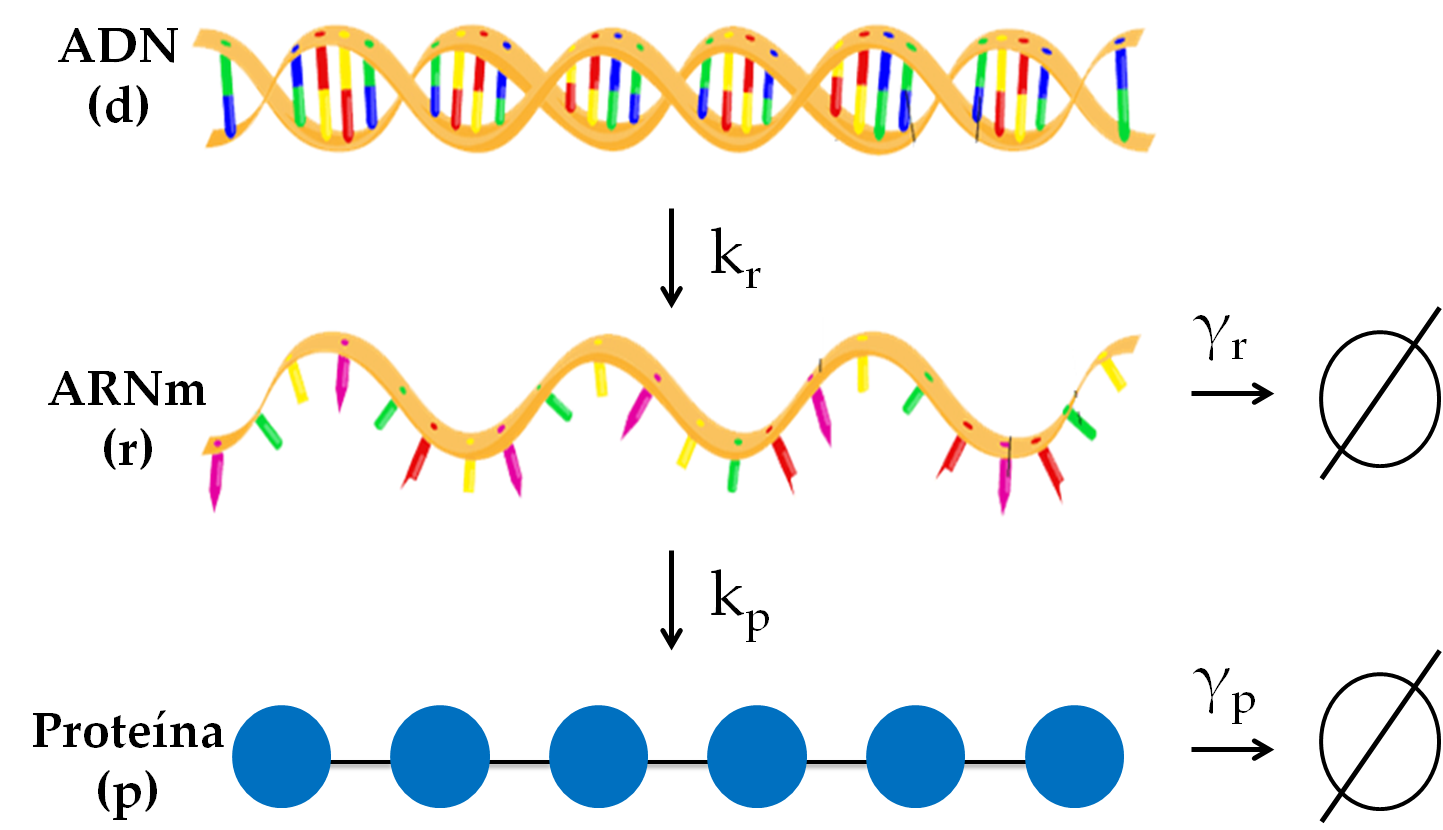
\includegraphics[width=10cm]{Pmas-dogma}
  \caption{\label{fig:con-dogma} Procesos involucrados en la expresi\'on gen\'etica.}
\end{figure}

Teniendo en cuenta lo anterior, las ecuaciones diferenciales que
satisfacen $r(t)$ y $p(t)$ son 

\begin{equation}
\label{eq:dif}
\begin{split}
\frac{\mathrm{d}}{\mathrm{d}t}r(t) &= k_r - \gamma_r r(t),\\
\frac{\mathrm{d}}{\mathrm{d}t}p(t) &= k_pr(t) - \gamma_p p(t).
\end{split}
\end{equation}

Estas ecuaciones tienen una soluci\'on anal\'itica:


\begin{equation}
\label{eq:det}
\begin{split}
r(t) &= \frac{k_r}{\gamma_r}\left(1-e^{-\gamma_rt}\right),\\
p(t) &= \frac{k_rk_p}{\gamma_r\gamma_p}\left[1-e^{-\gamma_pt}+\frac{\gamma_p}{\gamma_p+\gamma_r}\left(e^{-\gamma_pt}+e^{-\gamma_rt}\right)\right].
\end{split}
\end{equation} 

Sin embargo, ahora nos interesa considerar el aspecto
discreto (es decir, que el n\'umero de ARNm y proteinas solamente puede
tomar valores enteros) y aleatorio de este problema. 

Para resolver las ecuaciones num\'ericamente teniendo en cuenta el
car\'acter estoc\'astico de los  eventos se considera un peque\~no
intervalo $\Delta t$, en el cu\'al se evaluar\'a si ocurre alguno de
los eventos. 
La probabilidad de que ocurra alg\'un evento en un tiempo $\Delta t$
peque\~no es  

\begin{equation*}
P(\mathrm{evento}) = \mathrm{Tasa\ del\ evento}\cdot \Delta t
\end{equation*}

Por ejemplo, la probabilidad para que en un intervalo $\Delta t$ se
produzca una prote\'ina es $k_p\cdot r(t)\cdot\Delta t$, y
an\'alogamente para los dem\'as eventos. 

Para resolver las ecuaciones se deben generar n\'umeros aleatorios
en cada intervalo $\Delta t$ para evaluar si cada uno  de los eventos
ocurre (de manera similar a como hicimos para la marcha
aleatoria). Seg\'un los resultados se actualizan las cantidades de
ARNm y prote\'inas. Esto se repite hasta llegar a un tiempo final
$T_f$.   


\begin{parts}

\part[10] Escriba un archivo llamado \verb"genetica.py"
que contenga la definici\'on de la clase \verb"Expresion" que puede
inicializarse con los par\'ametros $k_r$, $k_p$, $\gamma_r$,
$\gamma_p$, $r_0 \equiv r(t=0)$, $p_0 \equiv p(t=0)$, $\Delta t$ y $T_f$. 
Los valores por defecto deben ser $k_r = 1
\frac{\text{ARN}}{\text{min}}$, $k_p = 60
\frac{\text{proteinas}}{\text{ARN} \cdot \text{min}}$, $\gamma_r =
\frac{1}{5} \frac{1}{\text{min}}$  y $\gamma_p = \frac{1}{30}
\frac{1}{\text{min}}$, $r_0 = 0$,  $p_0= 0$, $\Delta t=0.0003$
minutos y $T_f=150$ minutos.  


\part[20] Escriba una funci\'on llamada \verb"resuelve" dentro de
la clase \verb"Expresion" para solucionar las ecuaci\'ones diferencial de
manera estoc\'astica para cualquier valor de los par\'ametros
iniciales. 
La funci\'on debe generar las listas de tiempo,  n\'umero de ARN y
n\'umero de prote\'inas.  Estas listas deben ser parte de la clase
\verb"Expresion". 

\part[20] Escriba una funci\'on llamada \verb"grafica" dentro de la clase
\verb"Modelo" que realice gr\'aficas de $r(t)$ vs. $t$ y $p(t)$
vs. $t$ que deben ser guardadas en archivos de formato pdf llamados
\verb"r_t.pdf" y \verb"p_t.pdf". 
La funci\'on debe tomar como opci\'on un argumento booleano llamado
\verb"analitica" para elegir si se grafican o no las ecuaciones 
\eqref{eq:det} sobre la soluci\'on num\'erica.

\part[40] Escriba un c\'odigo en python llamado \verb"poblacion.py" que
utilice a la clase \verb"Expresion" {\bf solamente con las funciones
requeridas en los puntos anteriores} para 
\begin{itemize} 
\item (20 pt) resolver las ecuaciones $N = 200$ veces con los mismos
  par\'ametros iniciales y guardar en archivos de texto
  (\verb"r_poblacion.dat", \verb"p_poblacion.dat") el valor final de $r$ y
  $p$ para cada ejecuci\'on.      
\item (20 pt) hacer histogramas (por separado, guardados en
  archivos \verb"r_histograma.pdf" y \verb"p_histograma.pdf") para el
  n\'umero de ARN y uno para el n\'umero de prote\'inas.
  El histograma para el n\'umero de ARN debe incluir una comparaci\'on con el
  resultado ana\'litico esperado que es una distribuci\'on de Poisson
  dada por la ecuaci\'on.
  
\begin{equation*}
P(r) = \frac{\lambda^re^{-\lambda}}{r!},
\end{equation*}
con $\lambda = \frac{k_r}{\gamma_r}$. 
Para utilizar el factorial ejecute la funci\'on $\Gamma$ de tal forma que $\Gamma(r+1) = r!$. Esto se puede hacer de la siguiente manera:

\begin{verbatim}
import scipy.special as ssp
ssp.gamma(r)
\end{verbatim}
\bf{NOTA: Este c\'odigo debe funcionar para cualquier valor de los
  par\'ametros de inicializaci\'on de la clase \verb"Expresion".}

\end{itemize}

\end{parts}
\end{questions}




\end{document}

